\documentclass[tablesignature]{scrartcl}
\usepackage[utf8]{inputenc}
\usepackage[T1]{fontenc}
\usepackage{fixltx2e}
\usepackage{graphicx}
\usepackage{longtable}
\usepackage{float}
\usepackage{wrapfig}
\usepackage{soul}
\usepackage{textcomp}
\usepackage{marvosym}
\usepackage{wasysym}
\usepackage{latexsym}
\usepackage{amssymb}
\usepackage{hyperref}
\tolerance=1000
\usepackage{booktabs}
\usepackage[scaled]{beraserif}
\usepackage[scaled]{berasans}
\usepackage[scaled]{beramono}
\usepackage[usenames,dvipsnames]{color}
\usepackage{fancyhdr}
\usepackage{subfig}
\usepackage{listings}
\lstnewenvironment{common-lispcode}
{\lstset{language={HTML},basicstyle={\ttfamily\footnotesize},frame=single,breaklines=true}}
{}
\usepackage{paralist}
\let\itemize\compactitem
\let\description\compactdesc
\let\enumerate\compactenum
\usepackage[letterpaper,includeheadfoot,top=12.5mm,bottom=25mm,left=19mm,right=19mm]{geometry}
\pagestyle{fancy}
\providecommand{\alert}[1]{\textbf{#1}}

\title{Presenter Flow in Zambia}
\author{Percy}
\date{March 2012}

\begin{document}

\maketitle

% Org-mode is exporting headings to 3 levels.

\pagenumbering{roman}
\thispagestyle{fancy}
\renewcommand{\headrulewidth}{0pt}
\renewcommand{\footrulewidth}{1pt}
\lhead{}
\rhead{}
\chead{}
\lfoot{{Percy} <{nela.program@gmail.com}>}
\cfoot{}
\rfoot{\thepage}
\begin{abstract}
\vspace{5cm}
{\LARGE{\textbf{Abstract:\\}}}
Zambia is a piece of Conference Management Software.  This document is a ``How To'' guide assisting in the way of entering and keeping track of Presenters for the Zambia FFF-branch instance for your conference.  This is still a work in progress.
\end{abstract}
\newpage
\renewcommand{\headrulewidth}{1pt}
\chead{{Presenter Flow in Zambia}}
\tableofcontents
\listoftables
\listoffigures
\newpage
\pagenumbering{arabic}
\section{Introduction}
\label{sec-1}


  There is a certain pattern to the flow of dealing with presenters,
  whether they are sought after as Guest Of Honor, or as presenters on
  specific subjects, or as individuals that people have suggested, and
  how to get them successfully into Zambia.  This section of the
  documentation will be referencing some things only available to
  SuperLiaison individuals, so if you do not have that designation,
  this document might not be very useful to you in terms of work-flow,
  but it is always good to have an understanding on how things go on.
  Please do not let that deter you from enjoying this document.
\section{Entering Presenters}
\label{sec-2}


  There are two basic paths for entering Presenters into Zambia,
  either they are entered via outside suggestion (by someone, possibly
  the presenter themselves) when the call for presenters is open, or
  by someone on the Liaison Team entering their information, because
  negotiations by another channel of communications has happened.  If
  the presenter is already in the system, either said presenter or a
  member of the Liaison Team can indicate their interest without
  rentering their data. In this case, go directly to the next section.
\subsection{Ouside Suggestions}
\label{sec-2_1}

   
   Depending on your convention, many of the folks who are going to
   present either applied to do so (once you put the call for
   presenters) or are recommended by other folk.  Either way they
   will probably have been entered in the Brainstorm Suggest a
   Presenter form (\hyperref[BrainstormSuggestPresenter.php]{BrainstormSuggestPresenter.php}).

\begin{figure}[H]
\centering
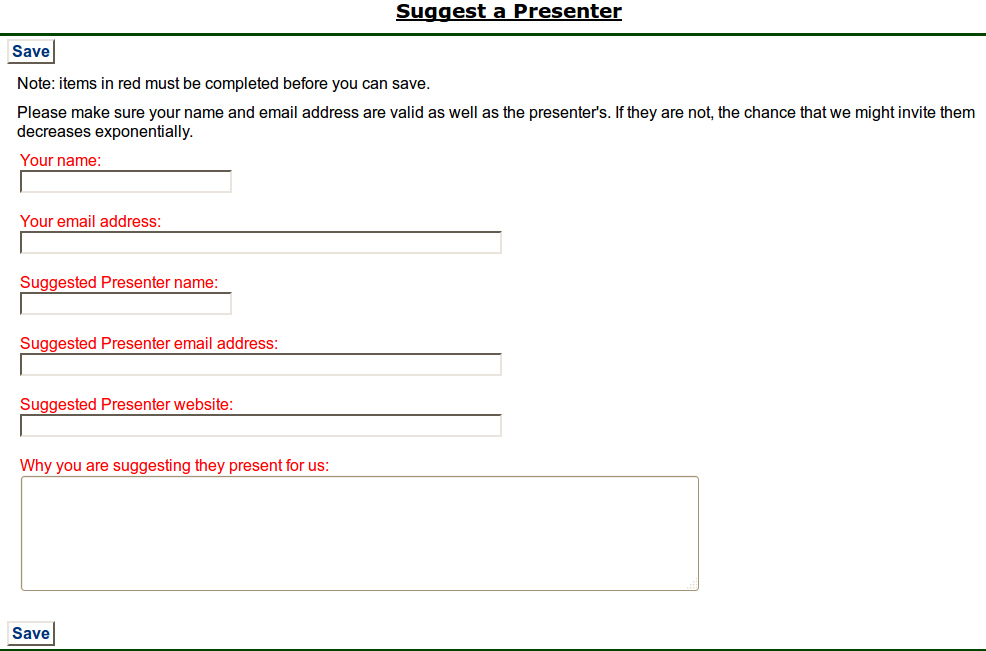
\includegraphics[width=0.98\textwidth]{./Images/Brainstorm_Suggest_Presenter.png}
\caption{\label{fig:Zambia_Presenter_Flow_Brainstorm_Suggest_Presenter}Brainstorm Suggest Presenter}
\end{figure}

   Fortunately or unfortunately, depending on the individual, you
   might not even have enough information to track them down and
   invite them but most people are good at putting in the
   information.  Once presenter information is entered, most of it
   will be in the ``NotesOnPresenter'' element, looking much like:

\begin{figure}[H]
\centering

\includegraphics[width=0.5\textwidth]{./Images/Notes_On_Participant.png}
\caption{\label{fig:Zambia_Presenter_Flow_Notes_On_Presenter}Notes On Presenter}
\end{figure}

   The element appears at the bottom of a presenter administration
   screen.

   Hopefully their name and email address will be in their profile
   should you desire to contact them.  Hopefully it will also include
   the email address of the submitter, so if the information they
   submitted doesn't actually connect you, or is incorrect, they will
   be helpful in facilitating the contact.
\subsection{By a Liaison person}
\label{sec-2_2}


   Often a Liaison person is tapped to enter in a participant because
   of negotiations done using other chanels.  Entering in the
   Presenter's information is slightly more comprehensive on the Enter
   Participant page (\hyperref[StaffEditCreateParticipant.php?action=create]{StaffEditCreateParticipant.php?action=create})
   which can also be found by going to the ``Manage Participant \&
   Schedule'' tab, and then choosing the ``Enter Participants'' link.


\begin{figure}[H]
\centering
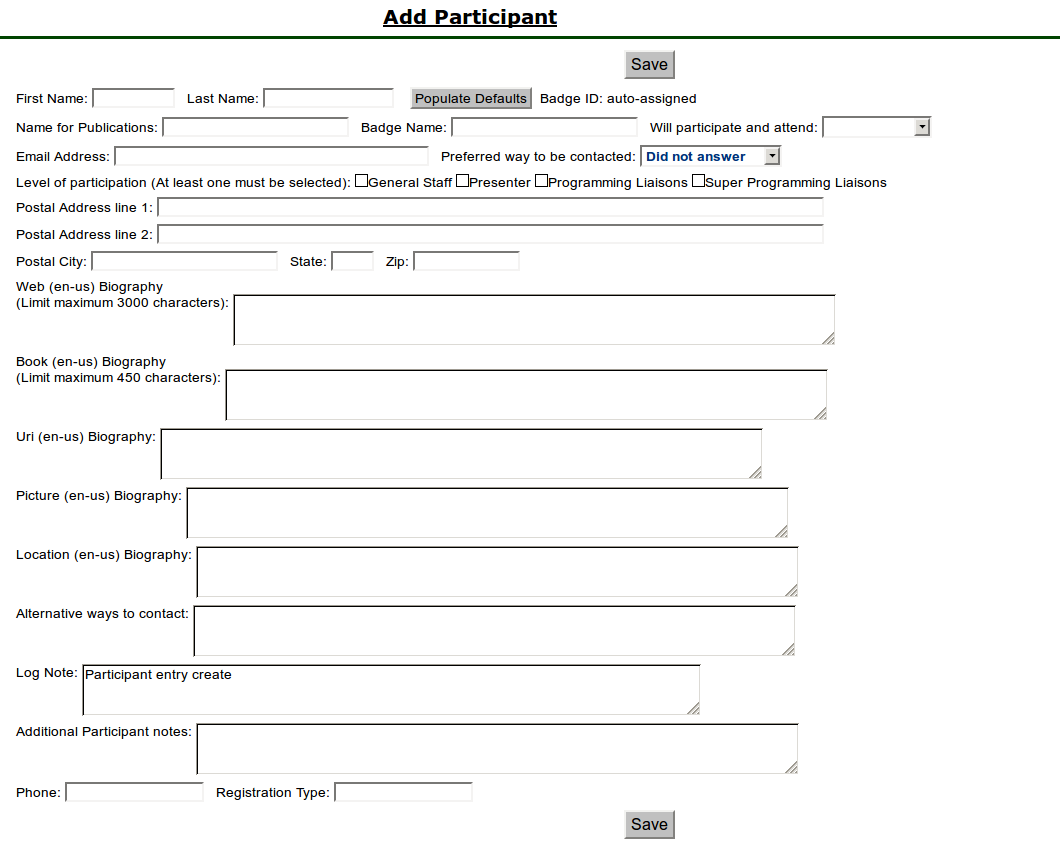
\includegraphics[width=0.95\textwidth]{./Images/Add_Participant.png}
\caption{\label{fig:Zambia_Presenter_Flow_Add_Participant}Add Participant}
\end{figure}

\begin{itemize}
\item In the names section, the first name, name for publications and
     badgename (the last two should be the same) are most
     important. The last name, although not mandatory, is often useful
     for disambiguation purposes.  The ``Populate Defaults'' button is
     mostly useless in our circumstances, being that it simply puts
     the first and last name in the publication and badge name
     fields.
\item The Will Participate and attend is very useful, but if you don't
     know their state it is acceptable to leave that blank for now.
     Unfortunately that will be problematic going forward beyond the
     compensation elements, for they won't show up in the pull-down
     menues until they are marked as ``Yes''.
\item It is important for the email address to be all in lower case.
\item Depending on the convention, the preferred way to be contacted
     may be limited.
\item Make sure that the ``Presenter'' box is checked.
\item The requirement level of the postal addresses for presenters is
     convention dependant.
\item The Biography elements are all the ``raw'' elements, i.e., what the
     presenter themselves can see and edit.  Depending on how your
     convention is organized, this might also be the final bio or it
     might have several different stages to go through before it is
     finalized.  The language in parentheses is only useful to note,
     if your convention is multi-lingual. (e.g., en-us is english,
     united states, fr-ca is french canadian)

\begin{itemize}
\item Web is the bio shared on the web.
\item Book is what is being put in the convention book.
\item URIs should be in fully-formed link format.
\item Pictures can be locally or remotely sourced.
\item Location should go away soon, don't worry about that.
\end{itemize}

\item The alternative ways of contact is always useful, if the
     presenters are willing to offer up one or more.  These can
     include other email addresses, contact info for support people,
     or other ways of being in touch with them.
\item The Log Note will also end up at the bottom of your page, with
     the rest of the Notes On Presenter elements.
\item Additional Participant notes are notes that follow their profile
     around.
\item Phone number is for contact, but depending on the strictures of
     your convention this might or might not be required.
\item Registration Type currently is a fill-in field that should be
     filled in with `PresenterComp'' but will become a pull-down list
     at some point.
\item Don't forget to hit the ``Save'' button, please.
\end{itemize}
\section{Updating Presenter Information}
\label{sec-3}

  
  Once in the system, the most common request by presenters is to have
  their password reset so that they can update the rest of their
  profile.  To do this, go to the Administer Participants link under
  the Manage Participants \& Schedule tab (\hyperref[AdminParticipants.php]{AdminParticipants.php}).
  Select the presenter from the drop-down menu and, once selected you
  may change their password, their interested and available setting,
  and their published name.

\begin{figure}[H]
\centering
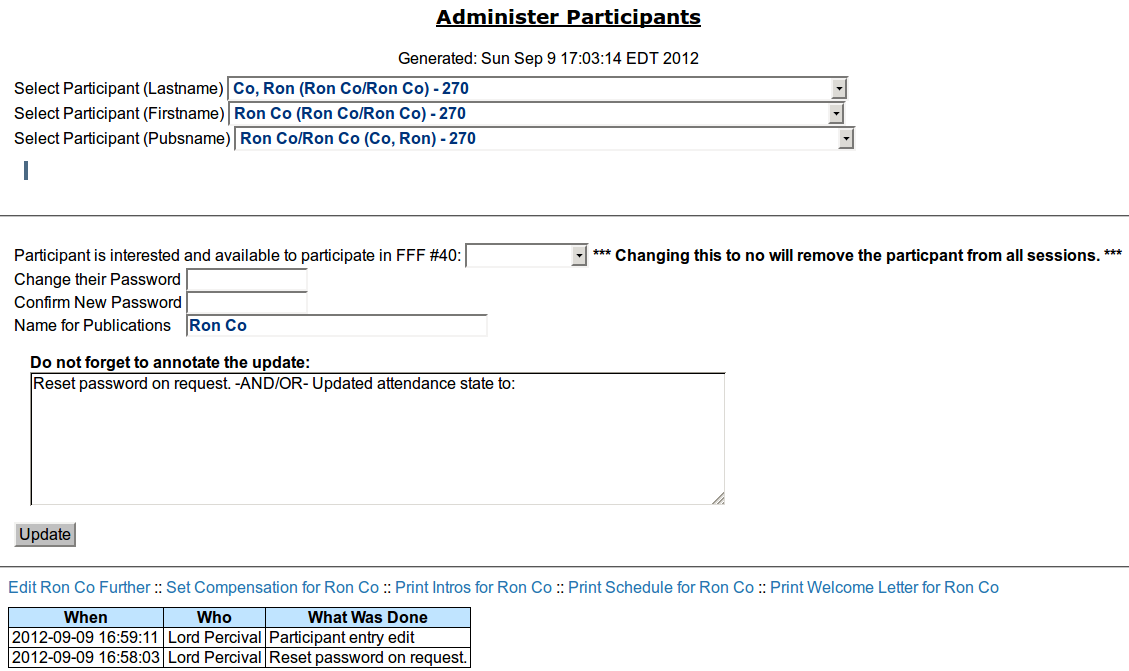
\includegraphics[width=0.95\textwidth]{./Images/Administer_Participants.png}
\caption{\label{fig:Zambia_Presenter_Flow_Administer_Participants}Administer Participants}
\end{figure}

  Most of the other modification pages won't have the presenter in the
  select menu until they are marked as a ``Yes'', as previously
  explained.  This is one of the pages that all the potential
  presenters are available in the pull-down menu.  If they are not
  available here, they might still be in the system, just not marked
  as someone you can see.  If you think they should already be in the
  system, and aren't showing up, please check with someone with
  greater permissions, or other div-heads.  They may already be in the
  system, just under another division.

  At the bottom of the Admin Participants page, there are several
  different links.  The next-most useful page is the first one: ``Edit
  PUBNAME further'' (\hyperref[StaffEditCreateParticipant.php?action=edit]{StaffEditCreateParticipant.php?action=edit}). When
  using the direct link, you will need to reselect the participant
  from the top of the page.

  This link will take you back to the page you should be familiar
  with, when you were creating the participant.  You can add to or
  change any of the extant information at this time.  If you want to
  see the importance of the fields, please see section 2.2 for diagram
  and instructions.
\section{Entering Compensation}
\label{sec-4}


  There are two ways to reach the place to enter Compensation for a
  Presenter.  One way is to go to the bottom of the Admin Participants
  page mentioned in the last section, then select the second link:
  ``Set Compensation for PUBNAME'' (\hyperref[StaffEditCompensation.php)]{StaffEditCompensation.php)} when
  using the direct link, you will need to reselect the participant
  from the top of the page.

\begin{figure}[H]
\centering
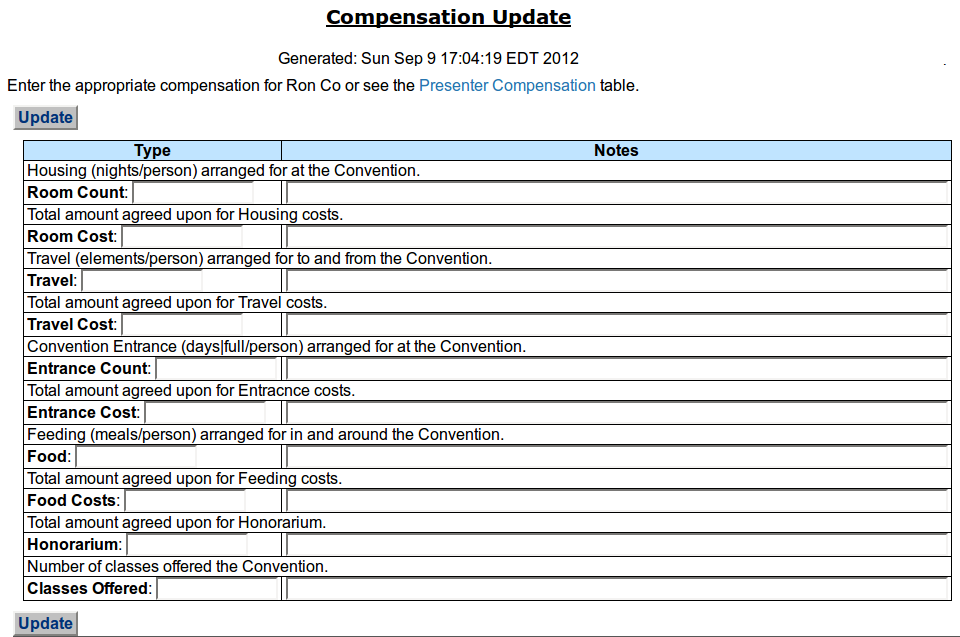
\includegraphics[width=0.98\textwidth]{./Images/Compensation_Update.png}
\caption{\label{fig:Zambia_Presenter_Flow_Compensation_Update}Compensation Update}
\end{figure}


  Only fill in the applicable compensation fields.  Please don't
  forget to hit ``Update'' before leaving the page.  Compensation is
  very conference dependant, please make sure any compensation entered
  is in lines with your conference's policies.

  You can also select the presenter name from the Presenter
  Compensation table (\hyperref[PresenterCompensation.php]{PresenterCompensation.php}).

\begin{figure}[H]
\centering
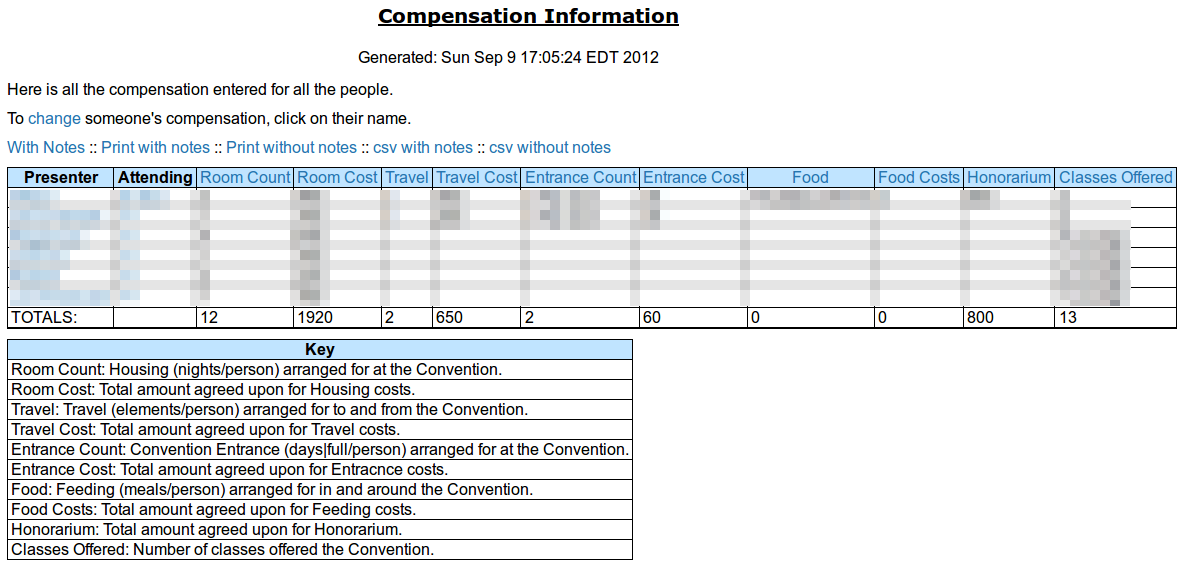
\includegraphics[width=0.98\textwidth]{./Images/Compensation_Information.png}
\caption{\label{fig:Zambia_Presenter_Flow_Compensation_Information}Compensation Information}
\end{figure}

  This table will fill in with the information entered.  The notes
  display makes it a very big table, hence the option without notes is
  the default.
\section{Entering Schedule Elements offered}
\label{sec-5}


  There are a few ways that Schedule Elements get entered into Zambia.
  A Schedule Element is anything that might end up on the schedule.
  This could be an Author Reading, a performance, a hosted meal, a
  class, a panel, a keynote speech, or anything else that is schedule
  worthy. 

  The information entered is visible to anyone who chooses to look at
  the website.  So people interested in what the decision process
  might be, or are looking to see if what they proposed is already
  under consideration, they can see much of the information.  This
  gives the community some sense of what is going on, so being
  descriptive about the information entered is a good thing.

  Once a Schedule Element is entered, if it is to be associated with a
  particular individual or set of individuals, that is done in several
  ways.
\subsection{Outside suggestion}
\label{sec-5_1}

   
   The Schedule Elements entered in from the outside, or by a
   presenter themselves, will have certain fields filled in, but not
   others.  Hopefully the submitter has given sufficient information
   in the form for you to determine if the Schedule Element is
   worthwhile, appropriate, or fits within this particular event.
   They might have also suggested a specific person for the Schedule
   Element.  The information asked for should be fairly
   straight forward. This is found on the Brainstorm screen under the
   Suggest a Session tab (\hyperref[BrainstormCreateSession.php]{BrainstormCreateSession.php}).

\begin{figure}[H]
\centering
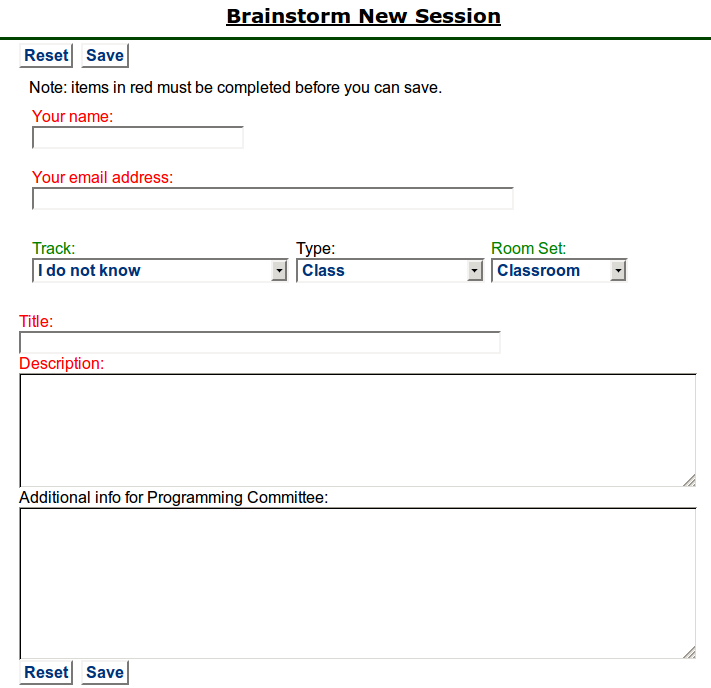
\includegraphics[width=0.98\textwidth]{./Images/Brainstorm_New_Session.png}
\caption{\label{fig:Zambia_Presenter_Flow_Brainstorm New Session}Brainstorm New Session}
\end{figure}
   
\subsection{By a Liaison person}
\label{sec-5_2}


   This form isn't overly complex, but there are some very important
   pieces here.  This can be found from the ``Create a New Session''
   link under the ``Manage Sessions'' tab (\hyperref[CreateSession.php]{CreateSession.php}).

\begin{figure}[H]
\centering
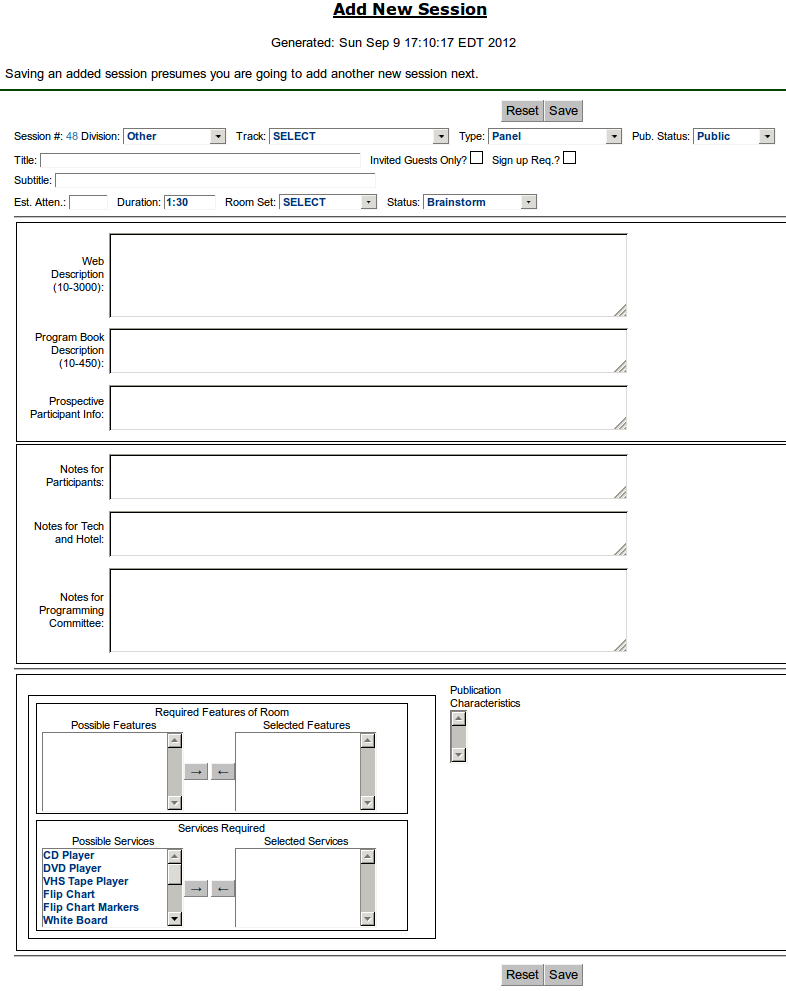
\includegraphics[width=0.98\textwidth]{./Images/Add_New_Session.png}
\caption{\label{fig:Zambia_Presenter_Flow_Add_New_Session}Add New Session}
\end{figure}

\begin{itemize}
\item The session number is just there for reference.  If the next step
     in your flow is to directly assign a person to a session, then
     note down the number for future reference (the next section).
\item Division: Most probably going to be ``Programming'' but other
     options are available.
\item Track: Finding the appropriate track is sometimes tricky if it
     falls into multiple categories.  You may want to set this to
     some variant of ``General'', or ``I don't know'', depending on the
     decision of your particular convention.
\item Type: What type of offering it is.  Often ``Panel'' or ``Class'' but
     might be something else.
\item Pub. Status (Publication Status): Describes if it is closed to a
     certain set of people, or only interesting to them, but most
     often will be ``Public''.
\item Title and Subtitle: Some conventions have limits on the length of
     these, and how they are published.
\item Invited Guests Only: If this is going to be given by a
     pre-scripted specific person, or set of people, this should be
     checked, so other presenters cannot sign up to present for this
     Schedule Element.  If it is unchecked, when Presenters look for
     the list of Schedule Elements they are able to sign up for, this
     Schedule Element will be amongst them.  This effects weather the
     Prospective Participant Info below, is seen.
\item Sign up Req.? (Sign up Required): This is in place in case any
     particular Schedule Element requires pre-con sign-up.
\item Est. Atten. (Estimated Attendance): This should be left blank,
     since it is part of the feedback and history of the Schedule
     Element after it is given.
\item Duration: This might be set by the convention, or might be
     dependant on the Schedule Element, type of Schedule Element, or
     many other things.  There should be a default time set here by
     your convention.  This may or may not contain the break
     between Schedule Elements, again depending on the decision of
     your particular convention.
\item Room Set: Most room-sets will be standarized by your convention,
     but sometimes a presenter has a particular preference that can
     be accommodated.  Most often ``class room'', ``theater'', or
     ``unspecified'' will be your choice.
\item Status: If you are just entering the Schedule Element, and it has
     not been previously negotiated as a Schedule Element that has
     been confirmed, please set it as ``Brainstorm''.  If it has been
     accepted as definitely happening, ``Vetted'' is the level it should
     be set to.
\item Web Description: This is the description of the Schedule Element
     that will be on the website, once it is scheduled. It is shared
     with the Brainstorm page until then. Because of this, please
     enter an accurate description of the Schedule Element.  There may
     be length constraints (on both ends) for the description.
\item Program Book Description: This is the description of the Schedule
     Element that will end up in the publications.  It doesn't need to
     be entered immediately (especially if the Schedule Element has
     not yet become ``Vetted''). There are probably has greater
     restrictions on the length, due to the web costing less for space
     than publications do.
\item Prospective Participant Info: This information gets shared with
     all the Presenters, if the Schedule Element is not restricted by
     the ``Invited Guests Only'' checkbox being checked.  This
     information is available in the area where Presenters may choose
     to sign up for this Schedule Element.  Things like ``need at least
     three years experience in the publishing field, from the
     publisher's point of view'' or the like would go in this field.
\item Notes for Participants: If you have yet to assign the Schedule
     Element to someone in the system who has said ``Yes'', then their
     name should be put in this field.  When Schedule Elements are
     actually vetted and scheduled, then this field should be any
     particular notes that will be shared with the presenter or
     presenters, in their schedule.
\item Notes for Tech and Hotel: This is any of the notes that will go
     to logistics, beyond the Features and Services requests below.
     Like ``will need to shift around the table, with the assistant on
     it, in the middle of the class''.
\item Notes for Programming Committee: If this was a Schedule Element
     submitted via the Brainstorm Submit a New Session (see above) then
     any notes not specifically in the Schedule Element description
     end up here.  If you want to put commentary here, notes about the
     Schedule Element, why it was requested, who saw it elsewhere, if
     it fits into multiple tracks, or the like, this is the place to
     make such notations.
\item Features and Services: These are pick-lists that you can choose
     various features of the room, or services that should be provided
     for the room, for the paricular Schedule Element.  Everything
     from a CD Player to a Flush Toilette should be covered here.  If
     it isn't covered here, add it to the ``Notes for Tech and Hotel''
     above. Should it be a regular enough addition, it will probably
     be added to the select boxes here.
\item Publication Characteristics: Originally a hold-over from before,
     but might now be used to indicate an expanded track conception of
     the Schedule Elements, for multi-tracked elements.
\item Please, do not forget to save your work, or you will be unhappy.
\end{itemize}
\subsection{By a Presenter}
\label{sec-5_3}

   
   The presenter is taken to the outside suggestion section and asked
   to fill out the form there.  It will have their name associated
   with it directly, as opposed to ``Idea Suggestion'' as the suggesting
   individual.  This will allow for the association between them and
   the Schedule Element to be clean and fast.
\subsection{Associating the Schedule Element with a Presenter}
\label{sec-5_4}


   Most conventions only want to assign Presenters to Schedule
   Elements, after said element has become vetted, but not all
   convetions work that way.

   If you want to assign a particular Schedule Element to an
   individual or group of Presenters, make sure said individual or
   group have already been set to ``Yes'' in terms of being willing to
   present for your convention.  The next step is to find the Schedule
   Element in question.

   One way is to look under the ``Manage Sessions'' tab at the View All
   Sessions link.  Find the Schedule Element, then select the link
   provided by the number (not the title).

   A second way is also under the ``Manage Sessions'' tab, using the
   link ``(Precis View With Links)''.  Find the Schedule Element, then
   select the link provided by the number (not the title).

   A third path to the Schedule Element in question is still under the
   ``Manage Sessions'' tab. Enter the noted session id number in the
   ``Session ID:'' box at the bottom of that screen and hit the ``Search''
   button.  This should bring up just one record (the record that you
   are expecting, hopefully), again simply select the link provided by
   the number (not the title).

   The fourth and fifth path presume that you have already marked the
   class as ``Vetted'', otherwise it will not show up for either of
   these.

   A fourth path is still under the ``Manage Sessions'' tab, using the
   ``Edit an Existing Session'' link.  Not only will this allow you to
   select your Schedule Element from the pull-down list of possible
   Schedule Elements and edit the information that might have changed
   since it was submitted, but also if you select the link provided by
   the ``Session \#'' number, you will be in the right place.

   A fifth path is under the ``Manage Participants \& Schedule'' tab,
   using the ``Assign participants to a session'' link
   (\hyperref[StaffAssignParticipants.php]{StaffAssignParticipants.php}) and choosing the Schedule Element
   from the pull-down menu at the top of the page.

   Once you are on the ``Assign Participants'' page with the correct
   Schedule Element, go to the bottom of the page where the ``Assign
   participant not indicated as interested or invited.'' pull-down menu
   is located and select the presenter applicable then hit the ``Add''
   button.  The presenter will now show up with their ``Assigned'' box
   checked.  If this particular Schedule Element has had other
   presenters invited, or had other presenters expressed interest in
   being part of this particular Schedule Element, that individual
   will also show up here.  They might have their Assigned box checked
   or not, if that Schedule Element has been associated with that
   individual.
\section{Choosing Schedule Elements}
\label{sec-6}


  Once all the potential Schedule Elements are in place, then comes
  the delight of choosing which elements will be part of your
  convention, when they will happen, and which will have to be
  left for other conventions.  This is mostly dependant on the path of
  each convention, and is therefore outside the scope of this document
  to dictate.  There are several useful reports that might help with
  this process, listed in the appendix.

\newpage
\appendix
\pagenumbering{Alph}
\section{Appendix}
\label{sec-7}

\begin{tiny}
\begin{longtable}{|l|l|l|}
\caption{Web Pages Referenced in this Document} \label{tbl:usefulpages}\\
\hline
 Page Name               &  Link                                          &  Description                                                      \\
\hline
\endhead
\hline\multicolumn{3}{r}{Continued on next page}\
\endfoot
\endlastfoot
\hline
 Suggest A Presenter     &  BrainstormSuggestPresenter.php                &  Used by non-con folks to suggest Participants.                    \\
 Create Participant      &  StaffEditCreateParticipant.php?action=create  &  Used to create a Participant from scratch.                        \\
 Administer Participant  &  AdminParticipants.php                         &  Used to set the password, attendence state, and pubsname only.    \\
 Edit Participant        &  StaffEditCreateParticipant.php?action=edit    &  Used to update a Participant's information.                       \\
 Edit Compensation       &  StaffEditCompensation.php                     &  Used to edit a Presenter's compensation package.                  \\
 Presenter Compensation  &  PresenterCompensation.php                     &  Used to display the compensation for all presenters compensated.  \\
 Suggest a Session       &  BrainstormCreateSession.php                   &  Used by non-con folks to suggest Schedule Elements                \\
 Create a New Session    &  CreateSession.php                             &  Used to create a Schedule Element from scratch.                   \\
 Assign Participants     &  StaffAssignParticipants.php                   &  Used to connect a Participant to a Schedule Element               \\
\hline
\end{longtable}

\end{tiny}

\begin{tiny}
\begin{longtable}{|l|l|l|}
\caption{Useful Reports} \label{tbl:usefulreports}\\
\hline
 Report Name        &  Link                                             &  Description                                                                                                              \\
\hline
\endhead
\hline\multicolumn{3}{r}{Continued on next page}\
\endfoot
\endlastfoot
\hline
 View All Sessions  &  genreport.php?reportname=ViewAllSessions         &  Shows all sessions, regardless of their status.                                                                           \\
 Session Notes      &  genreport.php?reportname=sessionnotes            &  Interesting info on a Session for sessions whose status is one of EditMe, Brainstorm, Vetted, Assigned, or Scheduled.     \\
 Picky People       &  genreport.php?reportname=conflictpickypeople     &  Show who the picky people do not want to be on a panel with and who they are on panels with.                              \\
 Too Few People     &  genreport.php?reportname=conflictunder3assigned  &  Scheduled sessions in division Program: If these are panels, you need at least 3 people. Other types require at least 1.  \\
 Assed V. Sched     &  genreport.php?reportname=conflictschedassn       &  These are sessions that are either in the grid and have no one assigned or vice versa.                                    \\
 Double Booked      &  gdenreport.php?reportname=conflictpartdup        &  Find all instances where a participant is scheduled to be in two or more places at once.                                  \\
 \# of sessions     &  genreport.php?reportname=conflictpartnums        &  Compare number of sessions participants requested with the number of which they were assigned.                            \\
\hline
\end{longtable}

\end{tiny}

  In point of fact, there turned out to be too many of them, for this
  sampling to be useful.  Please check the Conflict Reports and the
  Prog Reports Indicies on the Available Reports page.

\end{document}
